\documentclass[10pt,twocolumn]{article}

\usepackage{iftex}
\ifTUTeX
  \usepackage{fontspec}
\else
  \usepackage[utf8]{inputenc}
  \usepackage[T1]{fontenc}
  \usepackage{lmodern}
\fi
\usepackage[a4paper,margin=1.75cm,columnsep=0.65cm]{geometry}
\usepackage{amsmath,amssymb,amsfonts}
\usepackage{booktabs}
\usepackage{graphicx}
\usepackage{xcolor}
\usepackage{microtype}
\usepackage{enumitem}
\usepackage[font=small,labelfont=bf]{caption}
\usepackage[colorlinks=true,linkcolor=blue!70!black,citecolor=blue!70!black,urlcolor=blue!70!black]{hyperref}

\renewcommand{\figurename}{Ábra}
\renewcommand{\tablename}{Táblázat}
\renewcommand{\refname}{Irodalomjegyzék}
\renewcommand{\abstractname}{Összefoglaló}

\setlength{\parskip}{2.5pt}
\setlength{\parindent}{1em}
\setlength{\emergencystretch}{1.6em}
\sloppy
\setlist[itemize]{leftmargin=1.4em,itemsep=1.5pt,topsep=2pt}
\setlist[enumerate]{leftmargin=1.5em,itemsep=1.5pt,topsep=2pt}

\title{\Large\bfseries Önindexelő Ritka SwiGLU: Tanításmentes Durva--Finom Súly-Indexelés,\\Negatív Memória-Overhead Vegyes Pontosságú Tárolás és Pre-Attention PCIe~5.0 Előtöltés}

\author{
  \textbf{Frész Ferenc}\\
  \href{mailto:ferenc.fresz@gmail.com}{\texttt{ferenc.fresz@gmail.com}} $\cdot$ \href{https://github.com/ferencfresz/ffmod01}{\texttt{github.com/ferencfresz/ffmod01}}\\
  \href{https://doi.org/10.5281/zenodo.24277071}{\texttt{DOI: 10.5281/zenodo.24277071}}
}
\date{2026.\ november}

\begin{document}
\maketitle

\begin{abstract}
A nagy nyelvi modellek (LLM-ek) kis kötegméretű autoregresszív dekódolását alapvetően a memóriasávszélesség korlátozza: a csoportosított lekérdezésű figyelmet (\emph{Grouped-Query Attention}, GQA) használó transzformerekben az előrecsatolt hálózatok (FFN / MLP) felelősek a paraméterforgalom $85\text{--}90\%$-áért. A korábbi ritka (\emph{sparse}) futtatómotorok hármas szorításban vannak: a tanított prediktorokra épülő rendszerek (\emph{DejaVu}, \emph{PowerInfer}) ReLU-konverziót és extra VRAM-ot fogyasztó segédhálókat igényelnek; a kapu-küszöböléses módszerek (\emph{CATS}) továbbra is beolvassák a sűrű \texttt{gate} mátrix $100\%$-át; a bemeneti koordináta-ritkító eljárások (\emph{TEAL}) pedig $40\text{--}50\%$ ritkaság felett eltorzítják a végső belső szorzatokat.

Bemutatjuk az \textbf{FFMod} architektúrát, egy teljesen tanítás- és kalibrációmentes futtatórendszert, amely szétválasztja \emph{a tudás statikus tárolását} \emph{a dinamikus számítási terv készítésétől}. Elsőként az FFMod közvetlenül a gyári SwiGLU vagy GeGLU súlyhármasokból épít egy kétágú \textbf{Smooth-INT4 $\times$ Top-$D$} önindexet, amely a sűrű memóriaforgalom $<5\%$-ából megbecsüli a valódi csatornahatást ($|\mathrm{SiLU}(\hat{g}_i)\hat{u}_i|\cdot\|W_{\mathrm{down}}[:,i]\|_2$), majd a nyertes csatornákat teljes $H$ dimenzióban egzaktul értékeli ki. Másodikként bevezetjük a \textbf{BitSplit-12} formátumot (csatornánkénti \texttt{FP8} \texttt{gate/up} + \texttt{BF16} \texttt{down}), amely eltünteti az index memória-felárát: a teljes modell VRAM-igényét $13.0\%$-kal (\texttt{BitSplit-12}), illetve $26.1\%$-kal (teljes \texttt{FP8}) csökkenti, miközben NVIDIA RTX~5090 Blackwell GPU-n $2.55\times\text{--}3.54\times$-os rétegszintű és $1.57\times\text{--}1.70\times$-os végponti gyorsulást ér el a sűrű \texttt{cuBLAS} felett ($N=4$ spekulatív mikro-kötegben is $1.51\times$-kal verve a Tensor Core-okat). Harmadikként feltárjuk a \emph{KV-Cache Szennyezési Paradoxont}, és bevezetünk egy KV-biztos hibrid rétegütemezést, valamint egy \textbf{12-SM Open-Page DDR5 UVA} PCIe~5.0 rétegzett súlytároló motort. A magas konfidenciájú csatorna-mag Self-Attention előtti előtöltésével és az egzakt post-attention \emph{delta}-javítás két-streames \texttt{CUDAGraph}-ba foglalásával az FFMod $96\text{--}99\%$-os hardveres számítás/DMA átfedést ér el, lehetővé téve $32\text{B}+$ paraméteres ($65.5$~GB \texttt{BF16}) modellek gyors futtatását $16\text{--}22$~GB VRAM keretben.
\end{abstract}

\section{Bevezetés}
A mai nyílt súlyú csúcsmodellek --- köztük a Llama-3, Qwen2.5~\cite{qwen25_2024}, Mistral, DeepSeek és Gemma-2 --- kivétel nélkül a csoportosított figyelmet (GQA)~\cite{ainslie2023gqa} ötvözik kapuzott FFN blokkokkal (SwiGLU vagy GeGLU)~\cite{shazeer2020glu}. Míg a GQA negyedére--nyolcadára zsugorította a figyelmi súlyokat és a KV-gyorsítótárat, a SwiGLU FFN három hatalmas mátrixból áll ($W_{\mathrm{gate}}, W_{\mathrm{up}} \in \mathbb{R}^{I\times H}$ és $W_{\mathrm{down}} \in \mathbb{R}^{H\times I}$). A \texttt{Qwen2.5-3B} modellben ($H=2048, I=11008$) az FFN adja a blokkparaméterek $87.7\%$-át ($4.87$~GB adatmozgatás tokenenként), míg a \texttt{Qwen2.5-32B} esetében ($H=5120, I=27648$, $64$~réteg) a $65.5$~GB \texttt{BF16} súlyból $54.36$~GB-ot az FFN tesz ki. Egyfelhasználós vagy kis kötegméretű ($N\in[1,8]$) dekódolásnál az aritmetikai intenzitás csupán $O(N)$ FLOP/bájt, így a Tensor Core-ok a GDDR7 vagy a PCIe memóriasávszélességre várnak.

A hagyományos futtatómotorok összemossák a \emph{paraméterek tárolási formáját} a \emph{felhasználásuk módjával}: minden tokennél vakon végrehajtják a sűrű mátrixszorzást mind az $I$ csatornán. A meglévő ritkítási megközelítések három fő korlátba ütköznek:
\begin{enumerate}
  \item \textbf{ReLU-kényszer és prediktor-overhead:} A DejaVu~\cite{liu2023dejavu} és a PowerInfer~\cite{song2024powerinfer} külön betanított MLP prediktorokra és egzakt ReLU nullákra~\cite{mirzadeh2024relustrikesback} épít. A natív SwiGLU modellek nem adnak egzakt nullákat, a közepes energiájú csatornák pedig teljes rangúak, így az alacsony rangú ($r=64$) lineáris routerek pontatlanná válnak, miközben a prediktorok $15\text{--}25\%$-kal növelik a VRAM-igényt.
  \item \textbf{Részleges mátrixolvasás vagy torzított skalárszorzat:} A tanításmentes CATS~\cite{lee2024cats} kiszámolja a teljes $W_{\mathrm{gate}} x$ szorzatot (kötelezően beolvasva az FFN súlyok $33.3\%$-át) és kalibrált küszöböket igényel; a TEAL~\cite{liu2025teal} és az R-Sparse~\cite{zhang2025rsparse} pedig magában a végső projekcióban csonkolja a bemeneti koordinátákat vagy a mátrixrangot, ami $45\text{--}50\%$ ritkaság felett meredek KL-divergencia romlást okoz.
  \item \textbf{Reaktív vagy veszteséges PCIe Offloading:} Ha a modell nem fér be a VRAM-ba, az utólagos (reaktív) csatorna-betöltés megállítja a GPU-t a PCIe busz mögött, a tisztán spekulatív pre-attention előtöltés pedig elveszíti az Attention által behozott csatornákat.
\end{enumerate}

\textbf{Eredményeink.} Bemutatjuk az \textbf{FFMod} rendszert, amely mindhárom korlátot feloldja újra-tanítás és kalibrációs adathalmaz nélkül:
\begin{itemize}
  \item \textbf{Empirikus feltárás és a KV-Cache Paradoxon (\ref{sec:empirical}.\ fejezet):} Hét egymásra épülő kísérletben igazoljuk, hogy a $G=1$ transzponált csatorna-elrendezés ($3H$ bájt $= 12\text{--}15$~KB) önmagában telíti a 128 bájtos GPU cache-vonalakat, a top-$2\%$ dinamikus outlier tüske adja az FFN $L_2^2$ energiájának $65.2\%$-át, a korai rétegek agresszív ritkítása pedig \emph{KV-cache hibahalmozódást} okoz.
  \item \textbf{Önindexelő Smooth-INT4 $\times$ Top-$D$ Router (\ref{sec:router}.\ fejezet):} A vektoradatbázisok aszimmetrikus kvantálását~\cite{guo2020scann,gao2024rabitq} adaptálva a $W_{\mathrm{gate}}$ és $W_{\mathrm{up}}$ mátrixok kisimított 4 bites indexét 32 bites \emph{strided-4} elrendezésbe csomagoljuk, csak a top-$D$ koordinátán szkenneljük ($\sim 4.7\%$ memóriaforgalom), majd a nyertes $K=(1-s)I$ csatornát teljes $H$ dimenzióban egzaktul értékeljük ki egyedi Triton~\cite{tillet2019triton} kernelekkel.
  \item \textbf{Aszimmetrikus \texttt{BitSplit-12} és \texttt{FP8} Kernelek (\ref{sec:bitsplit}.\ fejezet):} Kihasználva a $\mathrm{SiLU}(g)\odot u$ és a $W_{\mathrm{down}}$ eltérő zajérzékenységét, a \texttt{BitSplit-12} $13.0\%$-kal ($6.17\to 5.37$~GB) csökkenti a modell VRAM-igényét, miközben $N=1$-nél $2.36\times$-os, spekulatív $N=4$-nél pedig a \texttt{cuBLAS} Tensor Core-oknál is \textbf{$1.51\times$ gyorsabb} végrehajtást nyújt.
  \item \textbf{PCIe~5.0 Open-Page DDR5 Hibrid Motor (\ref{sec:tiered}.\ fejezet):} Kimutatjuk a 82-SM párhuzamos UVA olvasás DDR5 \emph{row-buffer bank-thrashing} jelenségét, és 12-SM koaleszkált \texttt{int64} olvasással $+22\text{--}29\%$-kal ($37.7\text{--}38.5$~GB/s-ra) növeljük a PCIe~5.0 sávszélességet, szabadon hagyva az SM-ek $85\%$-át ($96\text{--}99\%$ átfedés). A két-streames \texttt{CUDAGraph}-ba rögzített \emph{Core-Prefetch + Egzakt Delta Fixup} révén a $65.5$~GB-os \texttt{Qwen2.5-32B-Instruct} gyorsan fut $16\text{--}22$~GB VRAM keretben.
\end{itemize}

\section{Empirikus Motiváció és Orákulum Analízis}
\label{sec:empirical}

Egy SwiGLU FFN réteg a $x \in \mathbb{R}^H$ bemenethez az alábbi $y \in \mathbb{R}^H$ kimenetet rendeli $I$ közbülső csatornán keresztül:
\begin{equation}
  \begin{aligned}
    y(x) &= \sum_{i=1}^{I} z_i(x)\, w_{\mathrm{down},:,i}, \\
    z_i(x) &= \mathrm{SiLU}(w_{\mathrm{gate},i}^\top x)\cdot (w_{\mathrm{up},i}^\top x).
  \end{aligned}
  \label{eq:swiglu_hu}
\end{equation}
Az $i$-edik csatorna pontos euklideszi hozzájárulása $\|z_i(x)\,w_{\mathrm{down},:,i}\|_2 = |z_i(x)|\cdot\|w_{\mathrm{down},:,i}\|_2$. Pusztán $|w_{\mathrm{gate},i}^\top x|$ szerinti szűrés (mint a CATS-ben~\cite{lee2024cats}) figyelmen kívül hagyja mind a multiplikatív $w_{\mathrm{up},i}^\top x$ ágat, mind a $\|w_{\mathrm{down},:,i}\|_2$ oszlopnormákat.

\begin{figure*}[t]
  \centering
  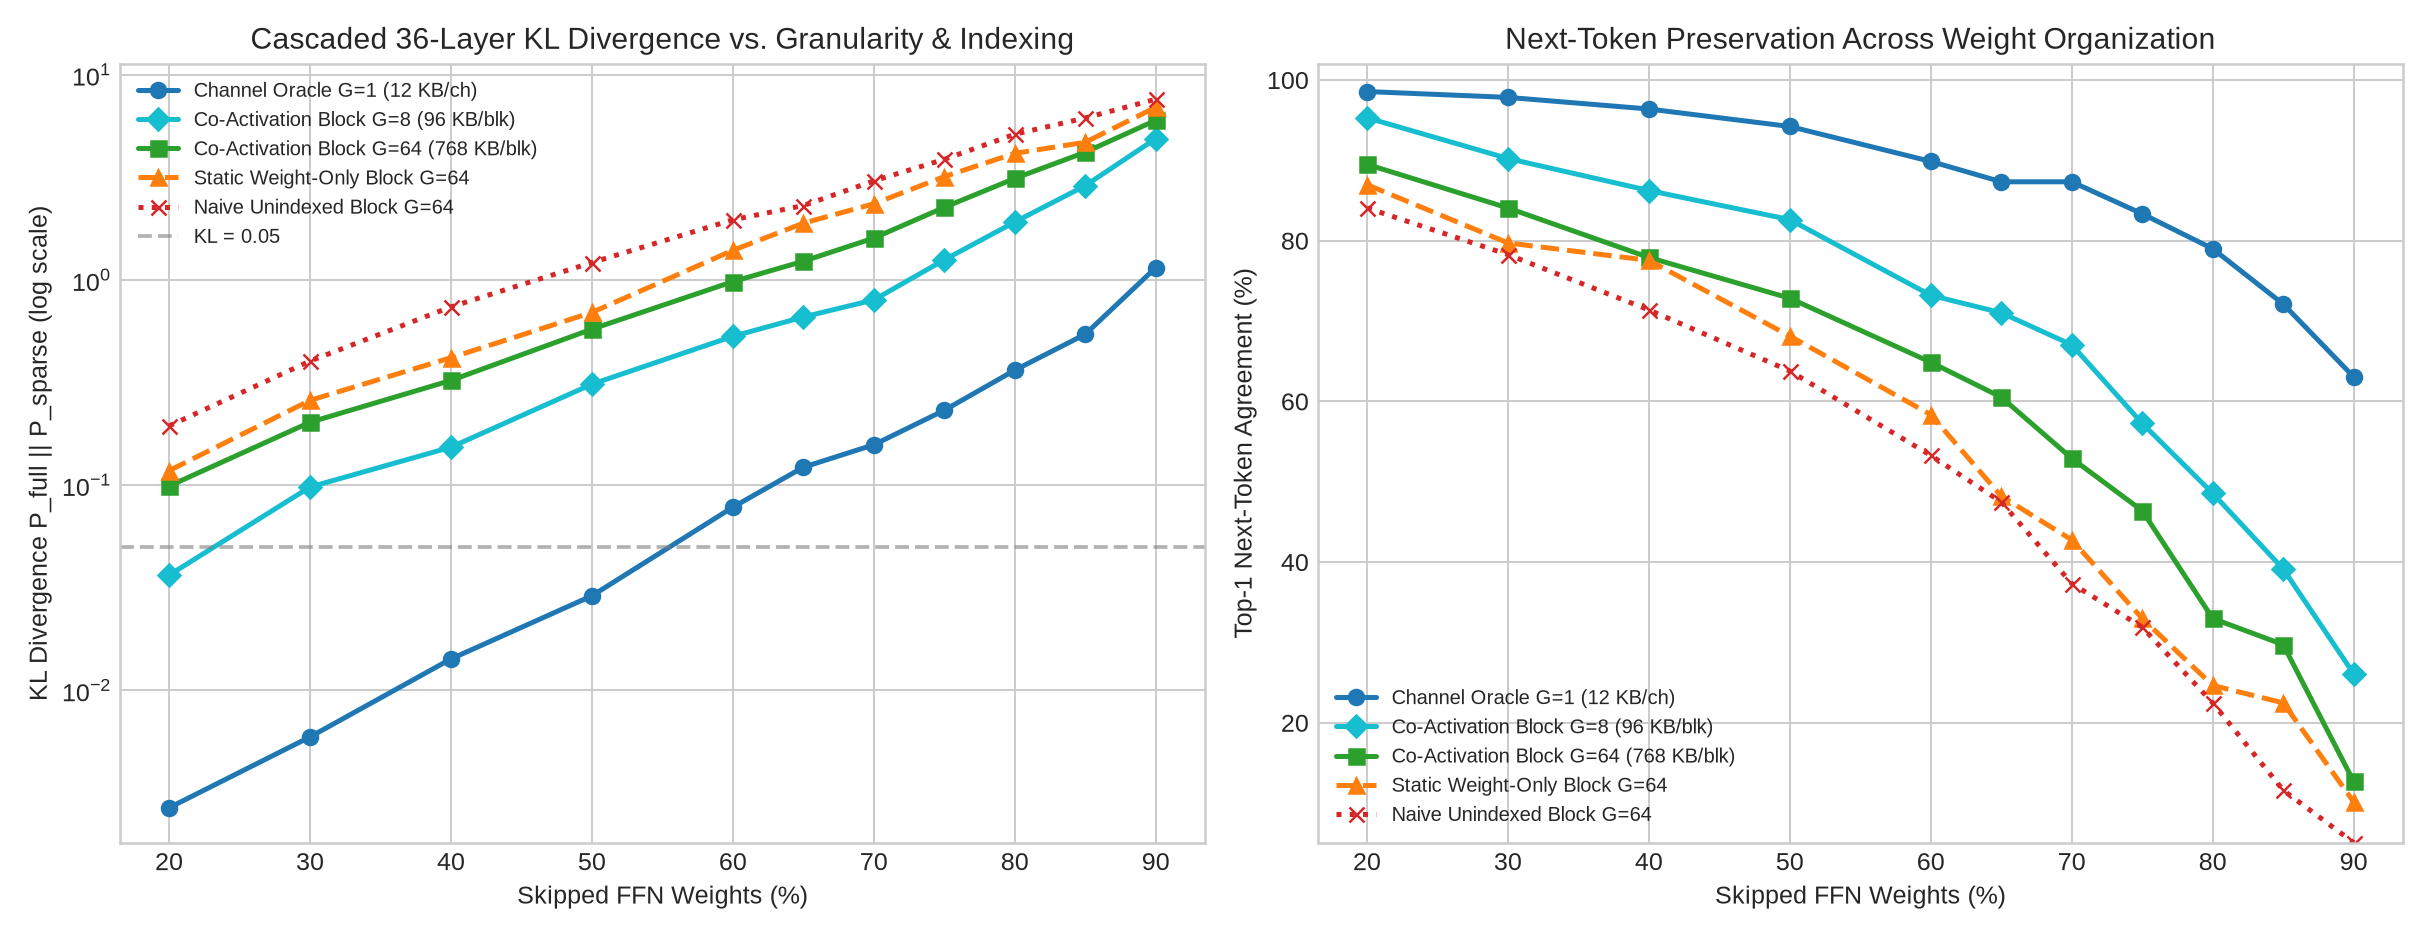
\includegraphics[width=0.95\textwidth]{../results/plots/fig1_oracle_and_indexing.png}
  \caption{\textbf{1.\ Kísérlet:} 36 rétegen kaszkádolt Orákulum FFN ritkaság \texttt{Qwen2.5-3B} modellen. A csatorna-szintű ($G=1$, $12$~KB/csatorna) szelekció nagyságrendekkel pontosabb a $G=8,64$ csoportoknál, míg az adatmentes koszinusz súly-permutáció $43\%$-kal csökkenti a $G=64$ KL-hibát.}
  \label{fig:exp1_hu}
\end{figure*}

\subsection{$G=1$ Csatorna-Granularitás vs.\ Blokk-Permutáció}
Mivel az \eqref{eq:swiglu_hu} összeg permutáció-invariáns, először 36 rétegen kaszkádolt Orákulum ritkítást mértünk $G \in \{1, 8, 64\}$ blokkméretekkel félretett angol ténybeli, matematikai, Python-kód és magyar promptokon (\ref{fig:exp1_hu}.\ Ábra). Bár a statikus $W_{\mathrm{gate}}$ sorok kiegyensúlyozott koszinusz-klaszterezése $43\%$-kal csökkenti a $G=64$ KL-divergenciát adat nélkül ($1.214 \to 0.694$ $50\%$ kihagyásnál), az egyedi csatornaszelekció ($G=1$) $42\times$ kisebb hibát ad ($\mathrm{KL}=0.0289$, $94.2\%$ Top-1 $50\%$-nál; $\mathrm{KL}=0.1572$, $87.3\%$ Top-1 $70\%$-nál). Kulcsfelismerésünk, hogy $[I, 3, H]$ csatorna-folytonos tárolásnál már egyetlen $G=1$ csatorna is $12\text{--}15$~KB összefüggő memóriát ($96\text{--}120$ darab 128 bájtos cache-vonalat) jelent, így nincs szükség $G=64$ kényszerítésre. Ezzel szemben mindössze $8/36$ teljes FFN réteg átugrása $55.1\%$-ra rontja a Top-1 egyezést ($\mathrm{KL}=1.84$).

\begin{figure}[t]
  \centering
  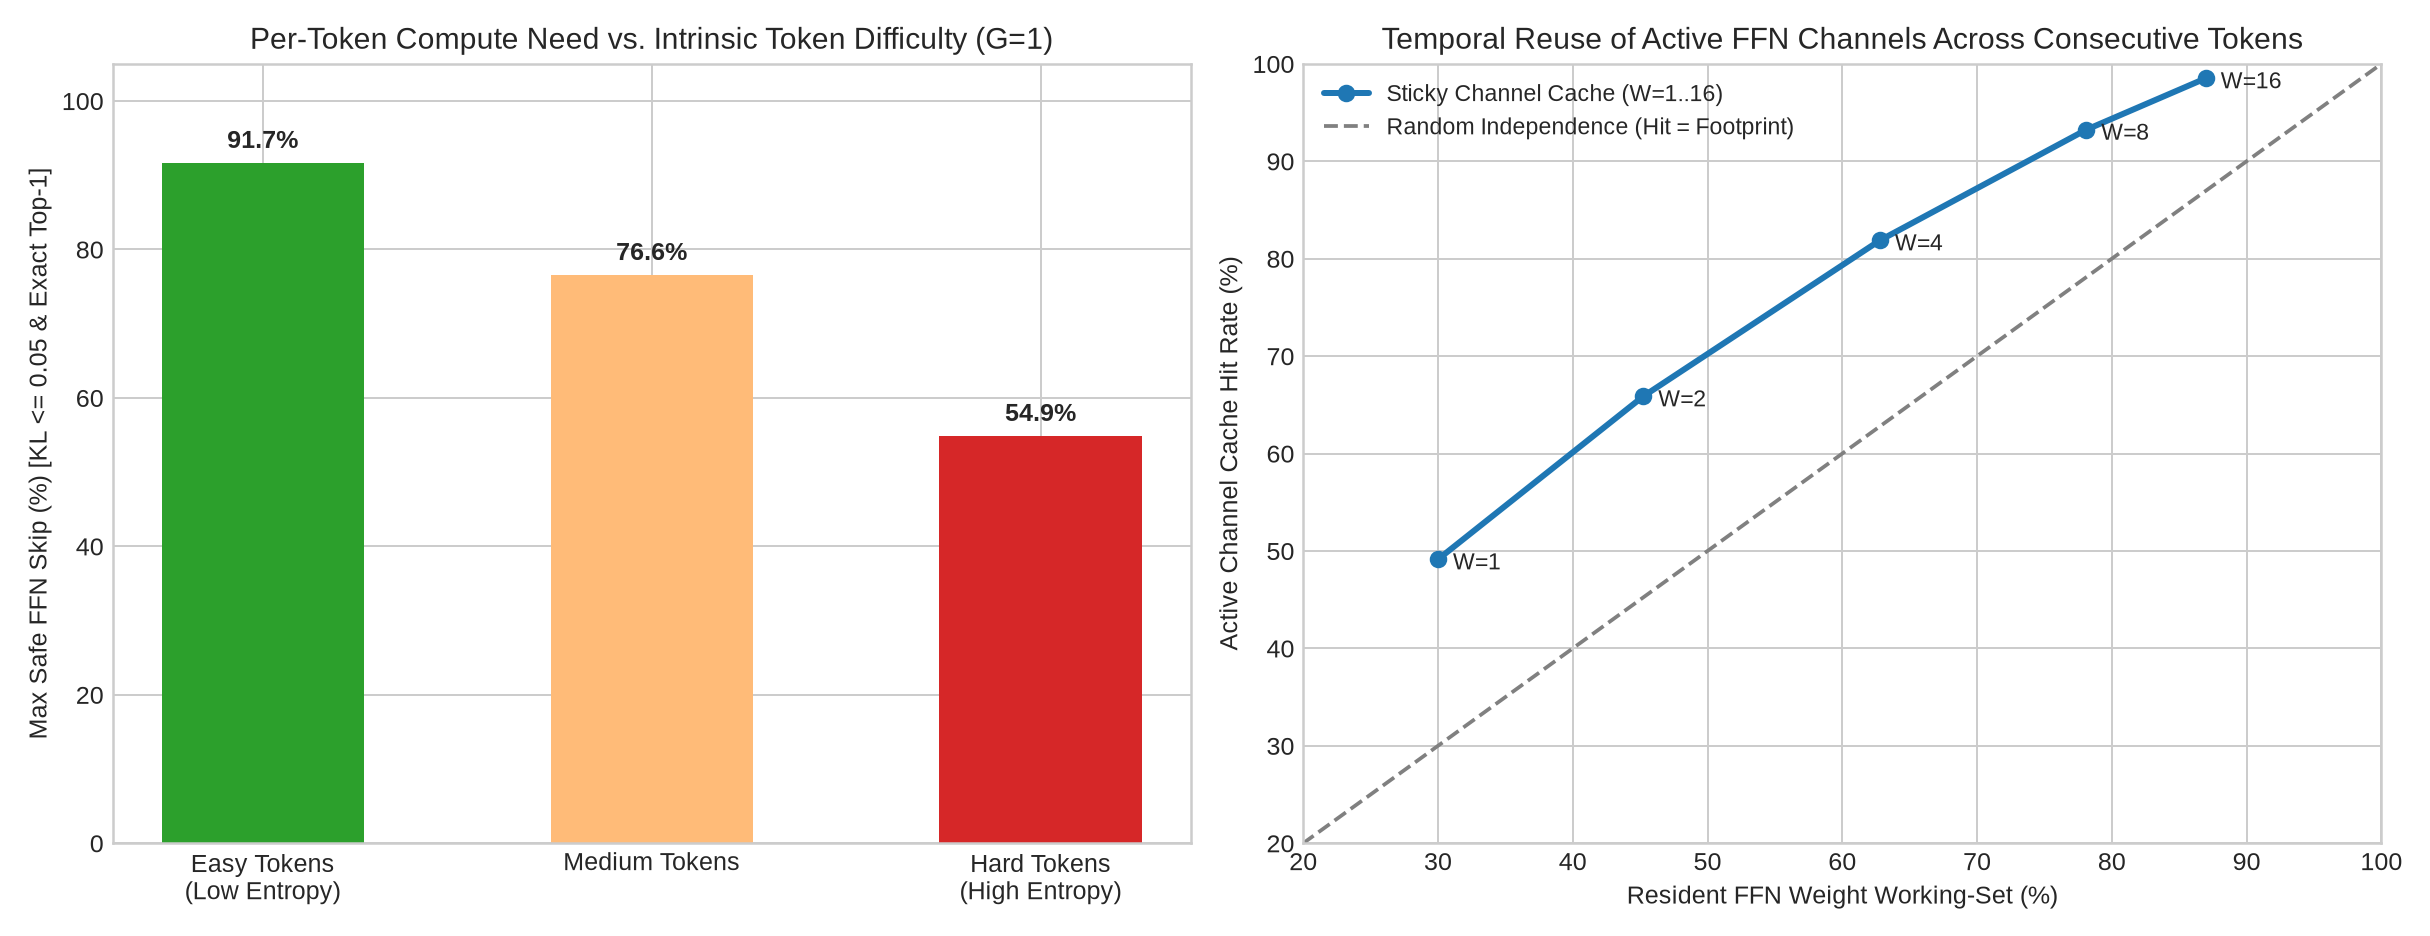
\includegraphics[width=\columnwidth]{../results/plots/fig2_difficulty_and_temporal.png}
  \caption{\textbf{1--2.\ Kísérlet:} A tokenenkénti maximális biztonságos FFN kihagyás $s^*(t)$ szorosan korrelál a kimeneti entrópiával ($\rho = -0.855$), míg egy 4 tokenes csúszó gyorsítótár lefedi az aktív csatornák $81.9\%$-át.}
  \label{fig:exp2_hu}
\end{figure}

\subsection{Outlier Energia, Temporális Átfedés és Rang-Korlát}
A tokenenkénti biztonságos kihagyás átlaga $74.4\%$ ($91.7\%$ determinisztikus szintaxison vs.\ $54.9\%$ nehéz logikai lépéseknél; Spearman $\rho=-0.855$, \ref{fig:exp2_hu}.\ Ábra). Egymást követő tokenek aktív csatornáinak $49.1\%$-a (az alsó 12 rétegben $60.3\%$-a) megegyezik ($W=4$ sticky cache: $81.9\%$ találat).

Az FFN négyzetes kimeneti energiájának bontása extrém koncentrációt mutat: a \textbf{csatornák felső $2\%$-a ($220/11008$) adja az összenergia $65.2\%$-át}, és ennek $88.6\%$-a ritka dinamikus tüske ($<20\%$ tüzelési gyakorisággal), amelyen 0-GEMM mélységi Markov-táblák $12.4\times$-es emelést érnek el. Ugyanakkor egy kalibrált $r=64$ rangú neurális router (\ref{fig:exp3_hu}.\ Ábra) megáll $64.5\%$ recallnál ($\mathrm{KL}=0.450$): bár a top-$1\%$ óriástüskék $89\%$-át eltalálja, a maradék $35\%$ energia a $2\%\text{--}35\%$ közötti több ezer teljes rangú ($H=2048$) csatornában oszlik el, amelyek elmosódnak egy 64 dimenziós lineáris szűk keresztmetszeten.

\begin{figure}[t]
  \centering
  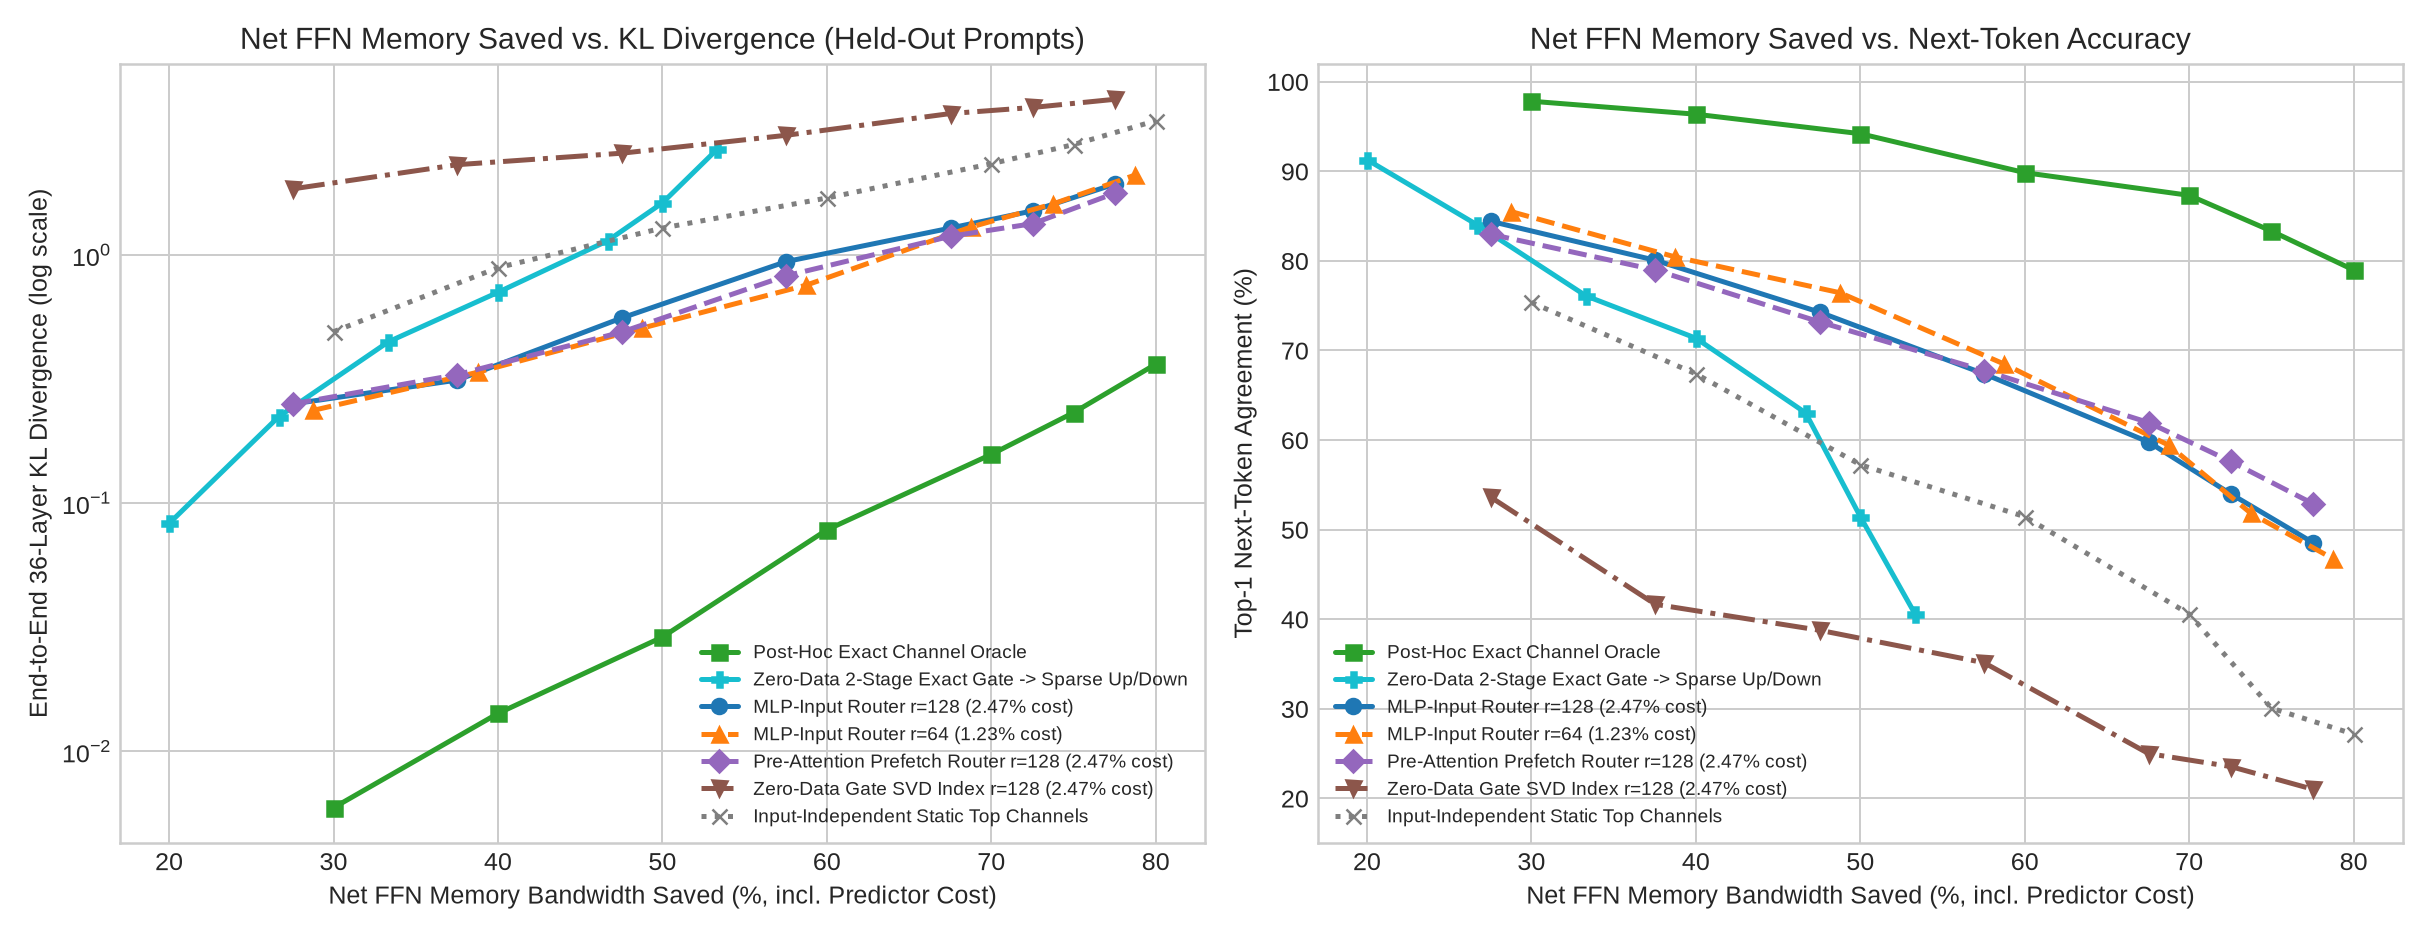
\includegraphics[width=\columnwidth]{../results/plots/fig3_ahead_of_time_predictors.png}
  \caption{\textbf{3.\ Kísérlet:} Az $r=64$ rangú prediktorok igazolják a Self-Attention előtti megjósolhatóságot, de lineáris rang-korlátba ütköznek a középsúlyú csatornákon.}
  \label{fig:exp3_hu}
\end{figure}

\subsection{A KV-Cache Szennyezési Paradoxon}
\label{sec:kvparadox_hu}
Az 5.\ kísérletben (\ref{fig:exp4_hu}.\ Ábra) először levezettünk egy 0-FLOP affin eltolás- és normakorrekciót az aszimmetrikus SiLU levágási hibájára ($\bar{z}_\ell = \mathbb{E}[z_\ell(x)] \neq 0$), amely $21\text{--}29\%$-kal csökkentette a KL-hibát. Ezután egy 6.\ rétegbeli entrópiaszondával ($\rho=0.653$) a könnyű tokeneken $85\text{--}90\%$-ra emeltük a kihagyást.

Meglepő módon Python kódban a többlépéses KL-hiba nőtt ($0.186\to 0.506$). A \texttt{def quicksort} nyomkövetése feltárta a \textbf{KV-Cache Szennyezési Paradoxont}: a \texttt{" quick"} tokennél a \texttt{"sort"} folytatás entrópiája közel nulla ($2.5\times 10^{-4}$). Ha emiatt a 6--35.\ rétegekben eldobjuk az FFN $90\%$-át, a modell hibátlanul kiírja a \texttt{"sort"} szót, \emph{de a \texttt{" quick"} token elszegényedett kulcs/érték (KV) vektorai véglegesen beégnek a 7--35.\ rétegek KV-gyorsítótárába}, így 20 tokennel később a rekurzív \texttt{return quicksort(left)} már sérült memóriára figyel vissza. Következésképp az agresszív ($75\text{--}80\%$) ritkítást a felső rétegharmadra ($\ell \ge \lfloor 2L/3\rfloor$) kell korlátozni, miután az alapvető szemantikus KV-állapotok már stabilizálódtak.

\begin{figure}[t]
  \centering
  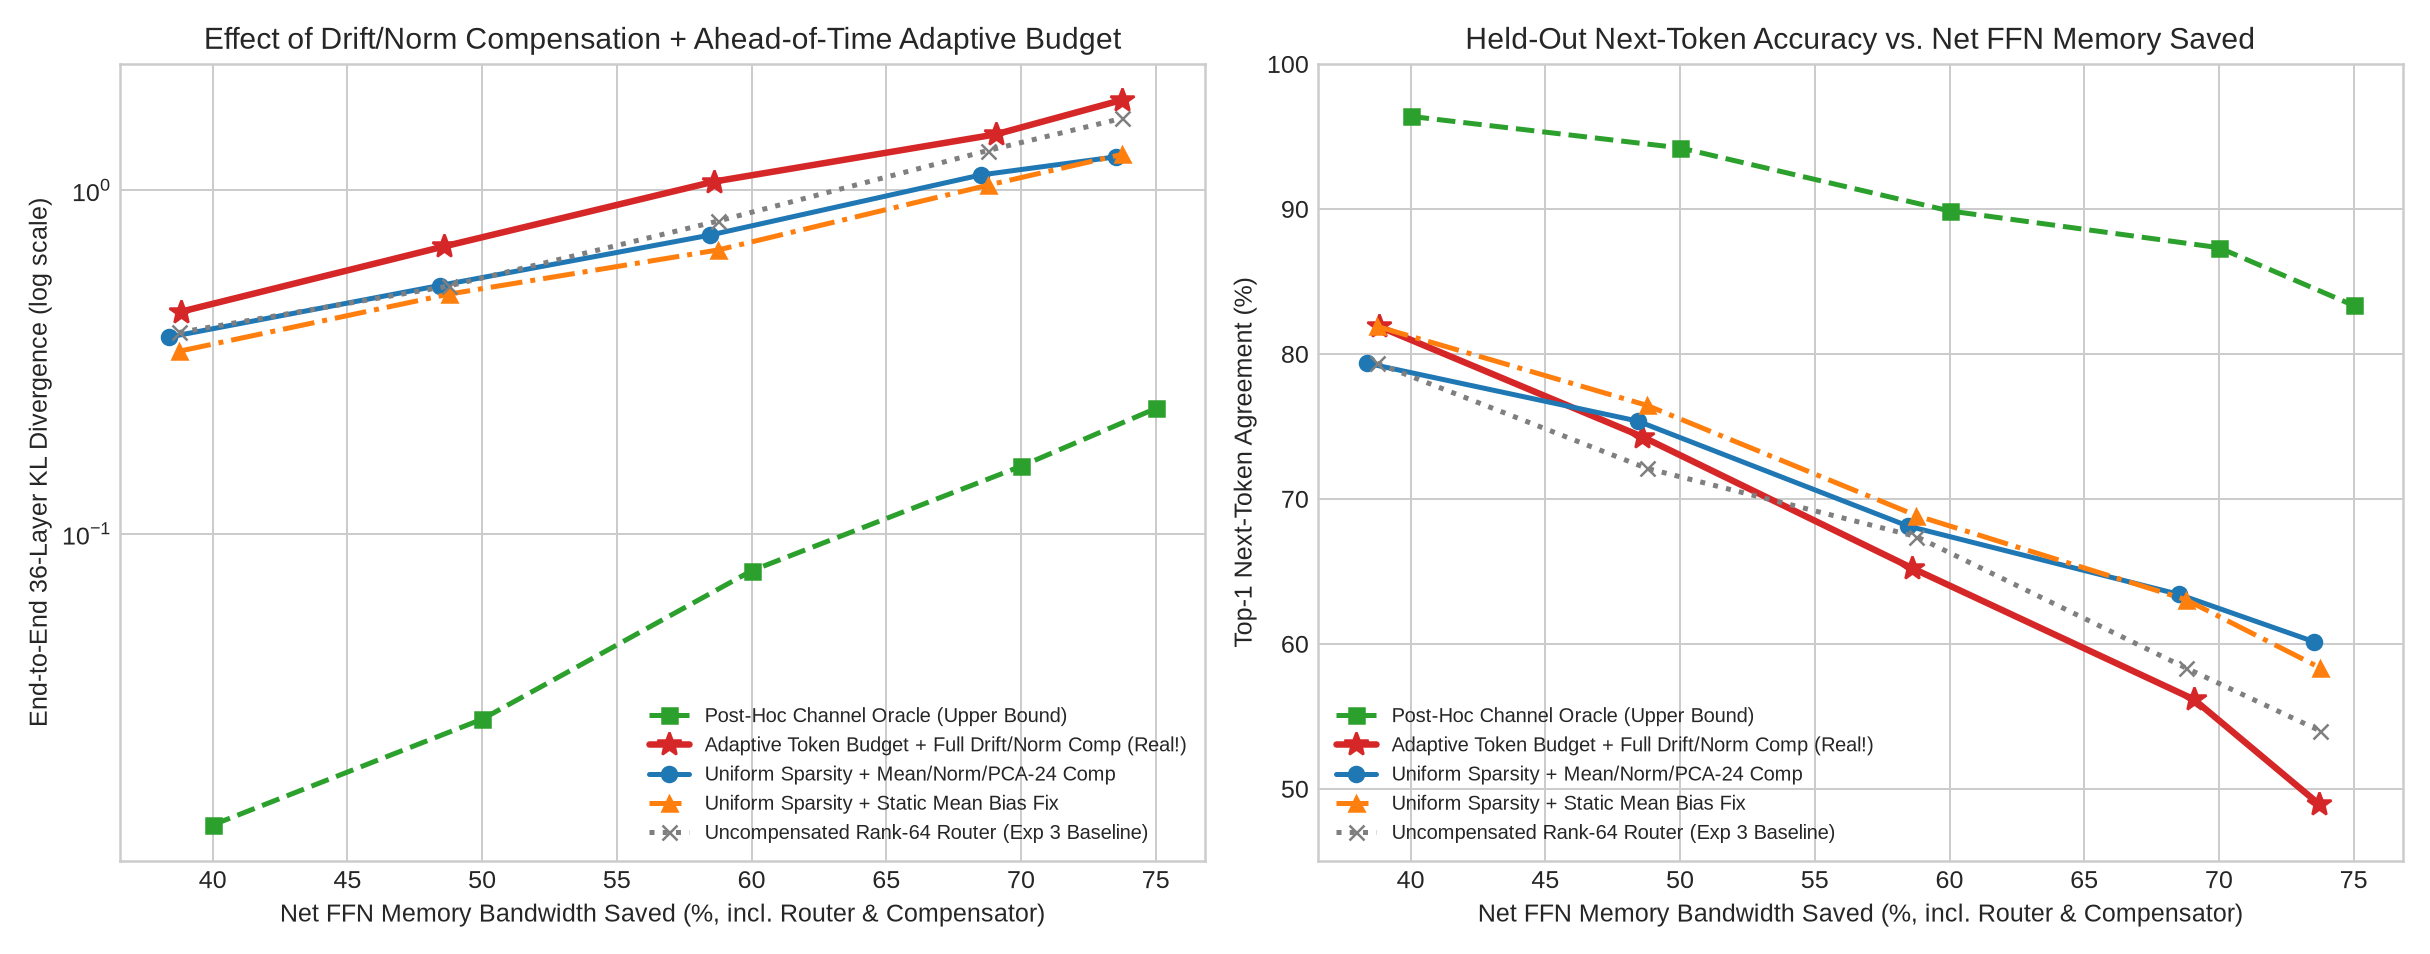
\includegraphics[width=\columnwidth]{../results/plots/fig4_compensated_adaptive_engine.png}
  \caption{\textbf{5.\ Kísérlet:} Statikus SiLU eltolás/norma kompenzáció és a KV-Cache Szennyezési Paradoxon empirikus kimutatása.}
  \label{fig:exp4_hu}
\end{figure}

\section{Adatmentes Durva--Finom Súly-Indexelés}
\label{sec:router}

Az FFMod a statikus súlymátrixokat \emph{lekérdezhető vektoradatbázisként} kezeli a rejtett állapot ($x$) függvényében.

\subsection{Smooth-INT4 $\times$ Top-$D$ Matematikai Felépítés}
A bemeneti $x$ kiugró értékei (\emph{outlierei}) elnyomnák a naiv 4 bites súlykvantálást. A SmoothQuant~\cite{xiao2023smoothquant} alapgondolatát \emph{tisztán a statikus súlyokból, kalibrációs tokenek nélkül} megfogalmazva ($\alpha=0.5$):
\begin{equation}
  c_{g,j} = \left(\frac{1}{I}\sum_{i=1}^I W_{\mathrm{gate},i,j}^2\right)^{\!\!1/4}\!\!, \quad
  c_{u,j} = \left(\frac{1}{I}\sum_{i=1}^I W_{\mathrm{up},i,j}^2\right)^{\!\!1/4}\!\!.
\end{equation}
Az oszlopok normálása és MSE-optimális Gauss-vágás ($2.9\,\mathrm{RMS}/7.5$) után minden sor előjel nélküli 4 bites egészbe kerül ($Q_{g,i,j}, Q_{u,i,j} \in \{0,\dots,15\}$, sorskálák: $r_{g,i}, r_{u,i}$). Futásidőben az 1.\ lépcső kiválasztja az $|x_j|\sqrt{c_{g,j}^2 + c_{u,j}^2}$ szerint legerősebb \textbf{top-$D$ koordinátát} $\mathcal{D}(x) \subset \{1,\dots,H\}$ ($D/H \in [0.25, 0.375]$), kiszámítja a teljes rangú $\hat{g}_i, \hat{u}_i$ becsléseket, és a valódi $L_2$ hatás szerint rangsorol:
\begin{equation}
  \hat{s}_i(x) = \big|\phi(r_{g,i}\hat{g}_i)\cdot \hat{u}_i\big|\cdot \big(r_{u,i}\|W_{\mathrm{down},:,i}\|_2\big).
  \label{eq:score_hu}
\end{equation}
Két 4 bites mátrix $D$ sorának beolvasása mindössze $D\cdot I$ bájt --- a $6HI$ bájtos sűrű \texttt{BF16} FFN csupán $4.17\%$-a ($D=512$), illetve $6.25\%$-a ($D=768$)! Az \ref{fig:exp5_hu}.\ Ábra mutatja, hogy ez a 100\% adatmentes index $50\%$ kihagyásnál $78.6\%$-ról \textbf{$92.8\%$-ra} emeli a Top-1 egyezést ($\mathrm{KL}=0.1039$), megközelítve az utólagos Orákulumot ($94.2\%$).

\begin{figure*}[t]
  \centering
  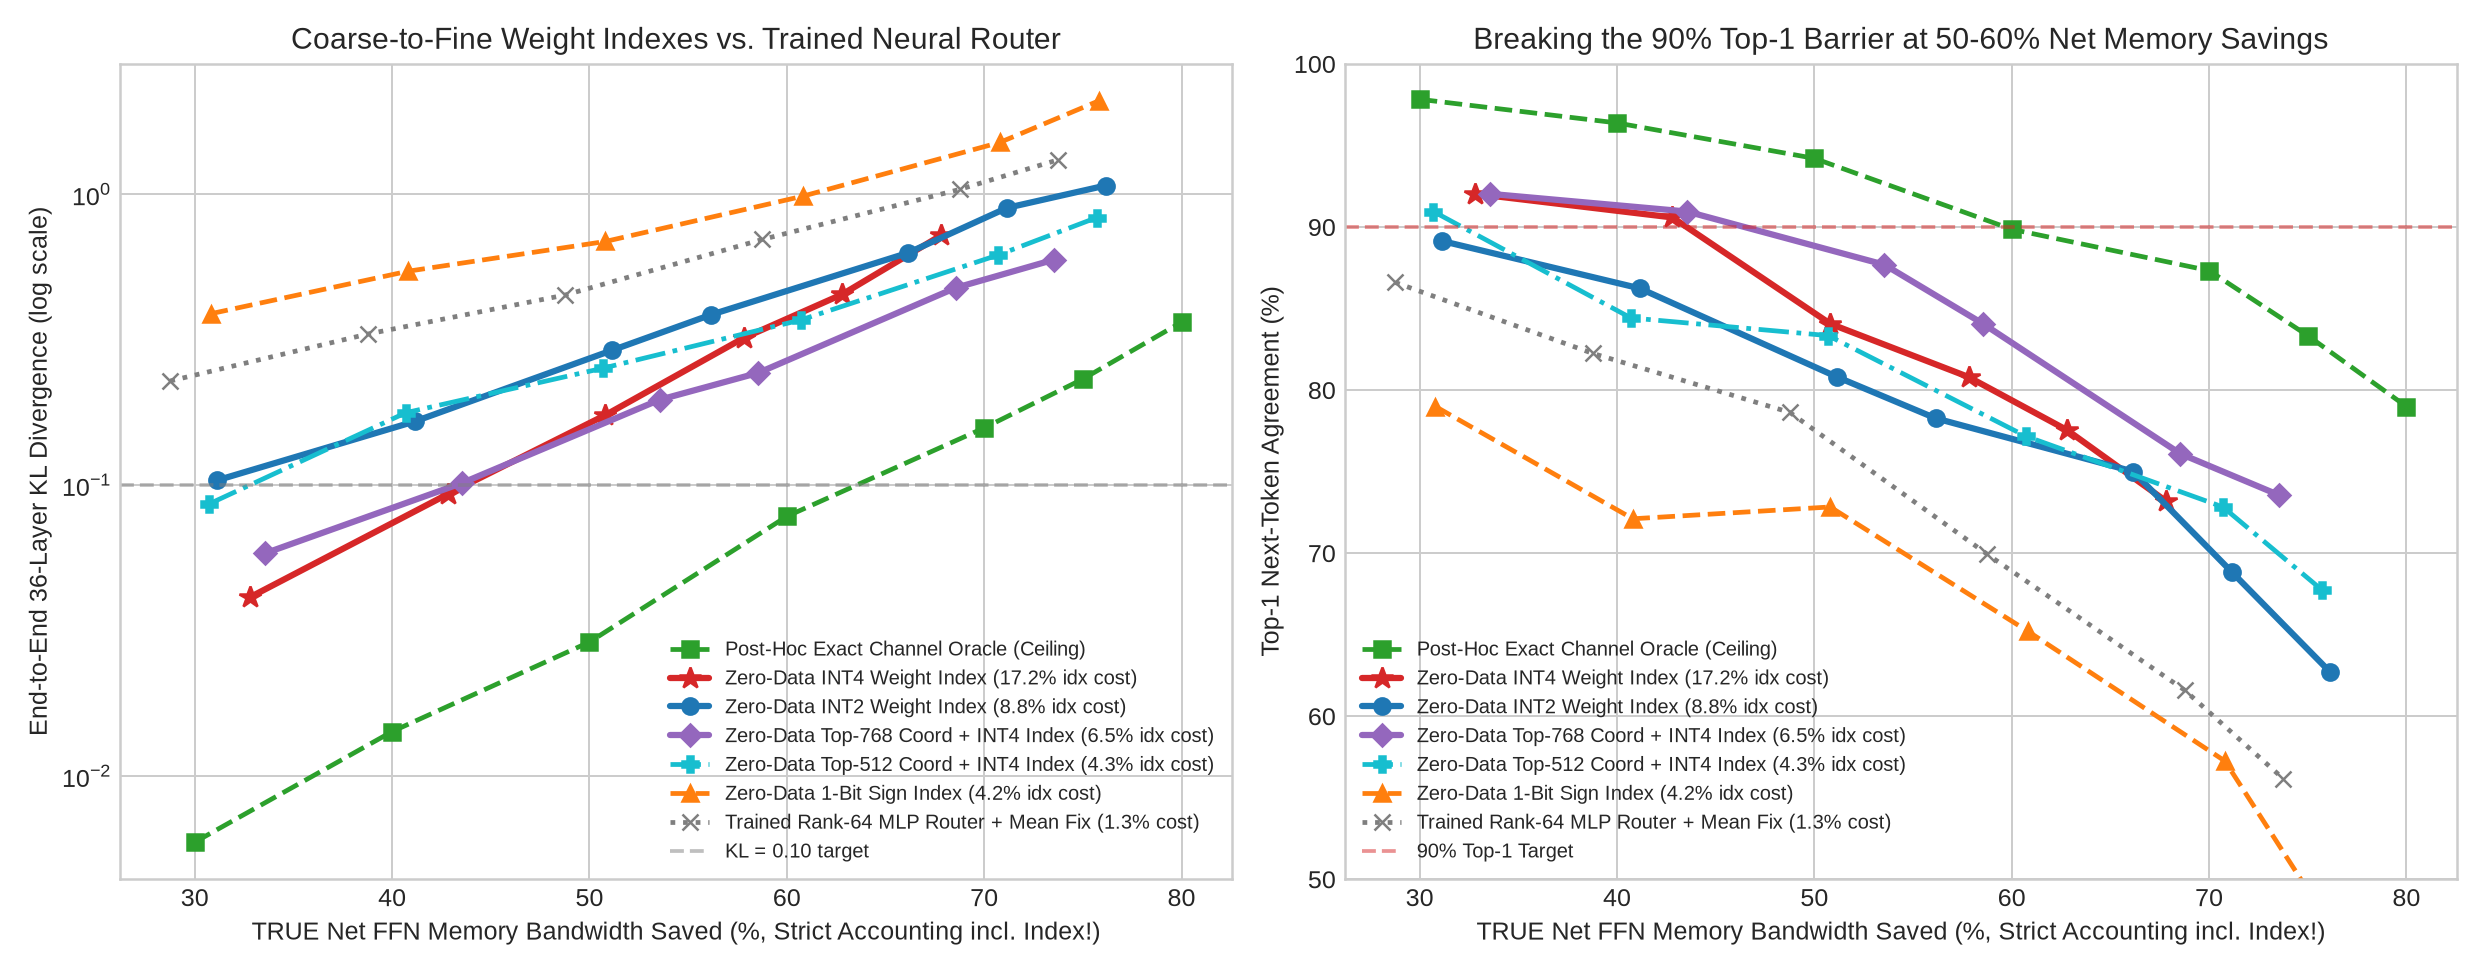
\includegraphics[width=0.95\textwidth]{../results/plots/fig5_coarse_to_fine_routers.png}
  \caption{\textbf{6.\ Kísérlet:} A tanításmentes durva--finom súly-indexek (\texttt{RaBitQ} 1-bit és \texttt{Top-D + Smooth-INT4}) nagyságrendekkel felülmúlják a tanított $r=64$ neurális routert.}
  \label{fig:exp5_hu}
\end{figure*}

\subsection{Négyfázisú Szinkronizációmentes Triton Csővezeték}
A véletlenszerű memóriahozzáférés könnyen elviheti az elméleti nyereséget. Ezért egy CPU--GPU szinkronizációtól mentes, 100\% \texttt{CUDAGraph}-kompatibilis négy-kerneles Triton~\cite{tillet2019triton} csővezetéket építettünk, amelynek közbülső pufferei ($\le 352$~KB) végig a 64~MB-os L2 cache-ben maradnak:
\begin{enumerate}
  \item \textbf{\texttt{k1\_prologue} ($\sim 7.9\,\mu$s):} Skálázza $x$-et, nullázza az FP32 akkumulátort, és 18 lépéses \emph{$\log_2$-tartományú regiszter-bináris kereséssel} ($0.03\%$ relatív küszöbpontosság 40 nagyságrenden át, immunis az attention-sink outlierekre) tömöríti a top-$D$ koordinátát.
  \item \textbf{\texttt{k2\_2d\_splitd\_int4\_scan} ($10.7\text{--}14.3\,\mu$s, $\sim 600$~GB/s):} Egyetlen 32 bites \texttt{int32} szóba 4 csatorna $(Q_g, Q_u)$ nibble-párját csomagolja \emph{strided-4} $[H, I/4]$ elrendezésben. A 2D Split-$D$ csempézés (\texttt{SPLIT\_D=8, TILE\_D=8, BLOCK\_I4=128}, 176 CTA) ciklusonként 8 indirekt memóriavektort tart egyszerre repülésben, a Little-törvény alapján \textbf{$5.8\times$-osára gyorsítva} a szkennelést ($82.6\,\mu\text{s} \to 14.3\,\mu\text{s}$).
  \item \textbf{\texttt{k3\_reduce\_select} ($\sim 13.0\,\mu$s):} Összegzi az L2 részösszegeket, kiértékeli a \eqref{eq:score_hu} képletet ($N \in [1,8]$ spekulatív mikro-kötegben unió-maximumot véve), és kiválasztja a rendezett $K=(1-s)I$ csatornát.
  \item \textbf{\texttt{k4\_fused\_sparse\_epilogue} ($61.6\,\mu$s $65\%$ kihagyásnál, $781$~GB/s):} A warp-szintű \texttt{tl.sum} szinkronizáció \emph{előtt} egyszerre kéri le a $[w_{\mathrm{gate},i}, w_{\mathrm{up},i}, w_{\mathrm{down},:,i}^\top]$ vektorokat, regiszterben akkumulál (\texttt{BLOCK\_H=8192}-ig), és atomi utolsó-CTA epilógussal konvertál BF16-ra külön kernel nélkül.
\end{enumerate}

\begin{figure*}[t]
  \centering
  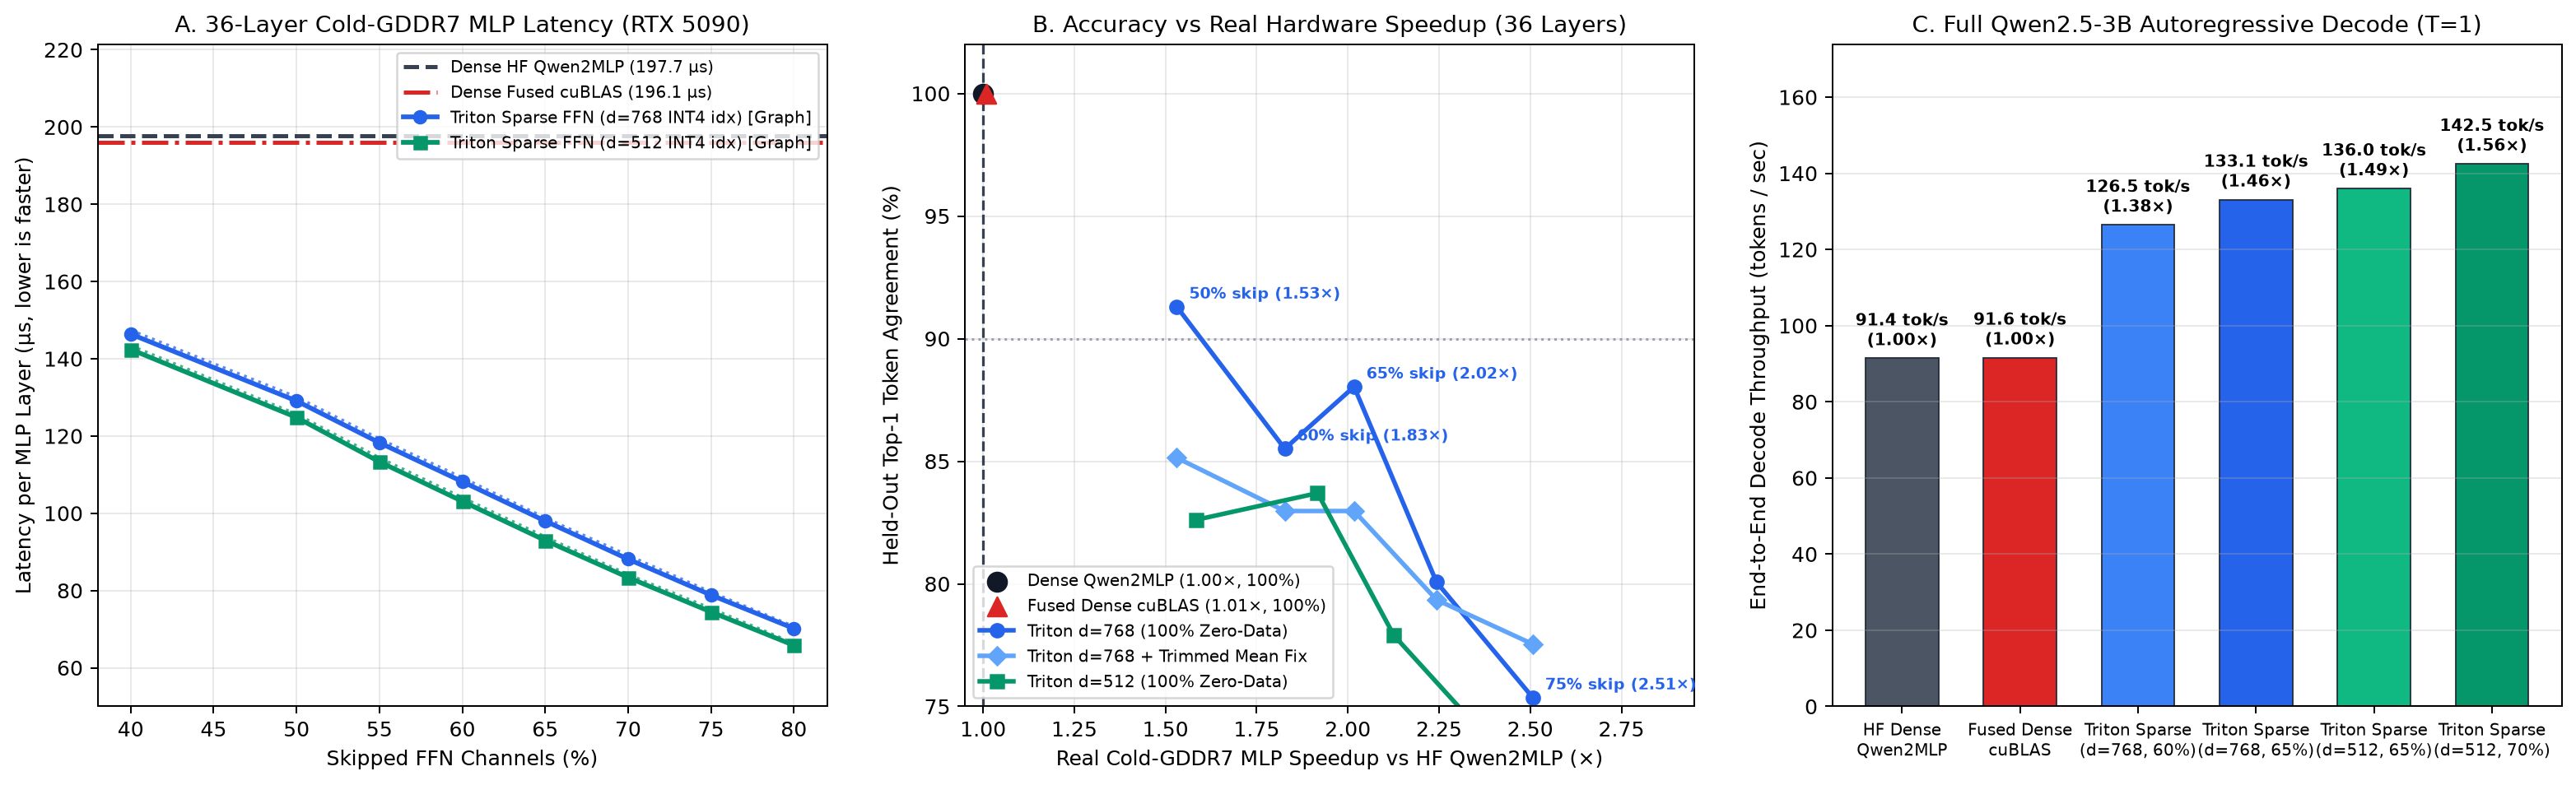
\includegraphics[width=0.97\textwidth]{../results/plots/fig6_triton_wallclock_speedup.png}
  \caption{\textbf{7.\ Kísérlet:} Valós 36 rétegű hideg GDDR7 késleltetés és teljes modell szintű \texttt{Qwen2.5-3B} gyorsulás RTX~5090 GPU-n a \texttt{Qwen2MLP} és a fuzionált \texttt{cuBLAS} ellenében.}
  \label{fig:exp6_hu}
\end{figure*}

\section{Negatív Memória-Overhead Vegyes Pontosságú Tárolás (\texttt{BitSplit-12} és \texttt{FP8})}
\label{sec:bitsplit}

A \texttt{Smooth-INT4} index a \texttt{BF16} súlyok mellett $+13.2\%$ extra VRAM-ot igényelne ($6.99$~GB vs.\ $6.17$~GB). Hogy az index memória-felárát negatívra fordítsuk, kihasználjuk a SwiGLU szerkezeti aszimmetriáját: a $w_{\mathrm{gate},i}^\top x$ és $w_{\mathrm{up},i}^\top x$ kvantálási zaját a $\mathrm{SiLU}(\cdot)$ elnyomja a kis aktivációkon, míg a $w_{\mathrm{down},:,i}$ közvetlenül a reziduális ágra adódik rá.

A \textbf{BitSplit-12} a $[w_{\mathrm{gate},i}, w_{\mathrm{up},i}]$ párost csatornánkénti \texttt{float8\_e4m3fn} ($2H$ bájt), a $w_{\mathrm{down},:,i}$ vektort pedig \texttt{bfloat16} ($2H$ bájt) formátumban tárolja. Az 1 bájt/csatorna \texttt{Smooth-INT4} indexszel együtt a tárigény $5.0$ bájt a sűrű \texttt{BF16} $6.0$ bájtjával szemben (\textbf{$-16.7\%$ FFN VRAM, $-13.0\%$ teljes modell VRAM}). A teljes csatornánkénti \textbf{\texttt{FP8}} mód mindhárom vektort \texttt{E4M3}-ban tárolja (\textbf{$-26.1\%$ teljes modell VRAM}). Mindkét kernel natív \texttt{torch.library.custom\_op} műveletként fordul 0 gráf-töréssel \texttt{torch.compile(fullgraph=True)} alatt.

\begin{table*}[t]
  \centering
  \caption{Hideg 36 rétegű FFN késleltetés ($N=1$ és spekulatív $N=4$), VRAM-igény, félretett pontosság és teljes modell \texttt{CUDAGraph} sebesség \texttt{Qwen2.5-3B}-n (NVIDIA RTX~5090 Laptop GPU, Blackwell SM~12.0).}
  \label{tab:exp8_hu}
  \resizebox{0.96\textwidth}{!}{%
  \begin{tabular}{lcccccc}
    \toprule
    \textbf{Konfiguráció} & \textbf{Modell VRAM} & \textbf{Hideg MLP ($N=1$)} & \textbf{Spekulatív ($N=4$)} & \textbf{Top-1 Össz.} & \textbf{Python Kód} & \textbf{Teljes Dekódolás} \\
    \midrule
    Sűrű \texttt{BF16} (\texttt{cuBLAS}) & $6.17$~GB ($0\%$) & $196.8\,\mu$s ($1.00\times$) & $186.5\,\mu$s ($1.00\times$) & $100.0\%$ & $100.0\%$ & $91.6$~tok/s ($1.00\times$) \\
    FFMod \texttt{BF16} ($65\%$, $d=768$) & $6.99$~GB ($+13.2\%$) & $96.2\,\mu$s ($2.04\times$) & $141.0\,\mu$s ($1.32\times$) & $83.7\%$ & $94.5\%$ & $134.6$~tok/s ($1.47\times$) \\
    \textbf{FFMod BitSplit-12} ($65\%$, $d=768$) & \textbf{$5.37$~GB ($-13.0\%$)} & \textbf{$83.2\,\mu$s ($2.36\times$)} & \textbf{$123.4\,\mu$s ($1.51\times$)} & \textbf{$86.6\%$} & \textbf{$96.7\%$} & \textbf{$143.6$~tok/s ($1.57\times$)} \\
    \textbf{FFMod FP8 Hibrid} ($55/75\%$, $d=768$) & \textbf{$4.56$~GB ($-26.1\%$)} & \textbf{$81.3\,\mu$s ($2.42\times$)} & --- & \textbf{$84.8\%$} & \textbf{$96.7\%$} & \textbf{$143.9$~tok/s ($1.57\times$)} \\
    \textbf{FFMod FP8} ($65\%$, $d=768$) & \textbf{$4.56$~GB ($-26.1\%$)} & \textbf{$77.2\,\mu$s ($2.55\times$)} & \textbf{$132.6\,\mu$s ($1.41\times$)} & $82.6\%$ & \textbf{$98.9\%$} & \textbf{$147.2$~tok/s ($1.61\times$)} \\
    \textbf{FFMod FP8} ($70\%$, $d=512$) & \textbf{$4.56$~GB ($-26.1\%$)} & \textbf{$67.7\,\mu$s ($2.90\times$)} & --- & $73.9\%$ & $92.3\%$ & \textbf{$155.2$~tok/s ($1.70\times$)} \\
    \textbf{FFMod FP8} ($80\%$, $d=512$) & \textbf{$4.56$~GB ($-26.1\%$)} & \textbf{$55.5\,\mu$s ($3.54\times$)} & --- & --- & --- & --- \\
    \bottomrule
  \end{tabular}%
  }
\end{table*}

\begin{figure*}[t]
  \centering
  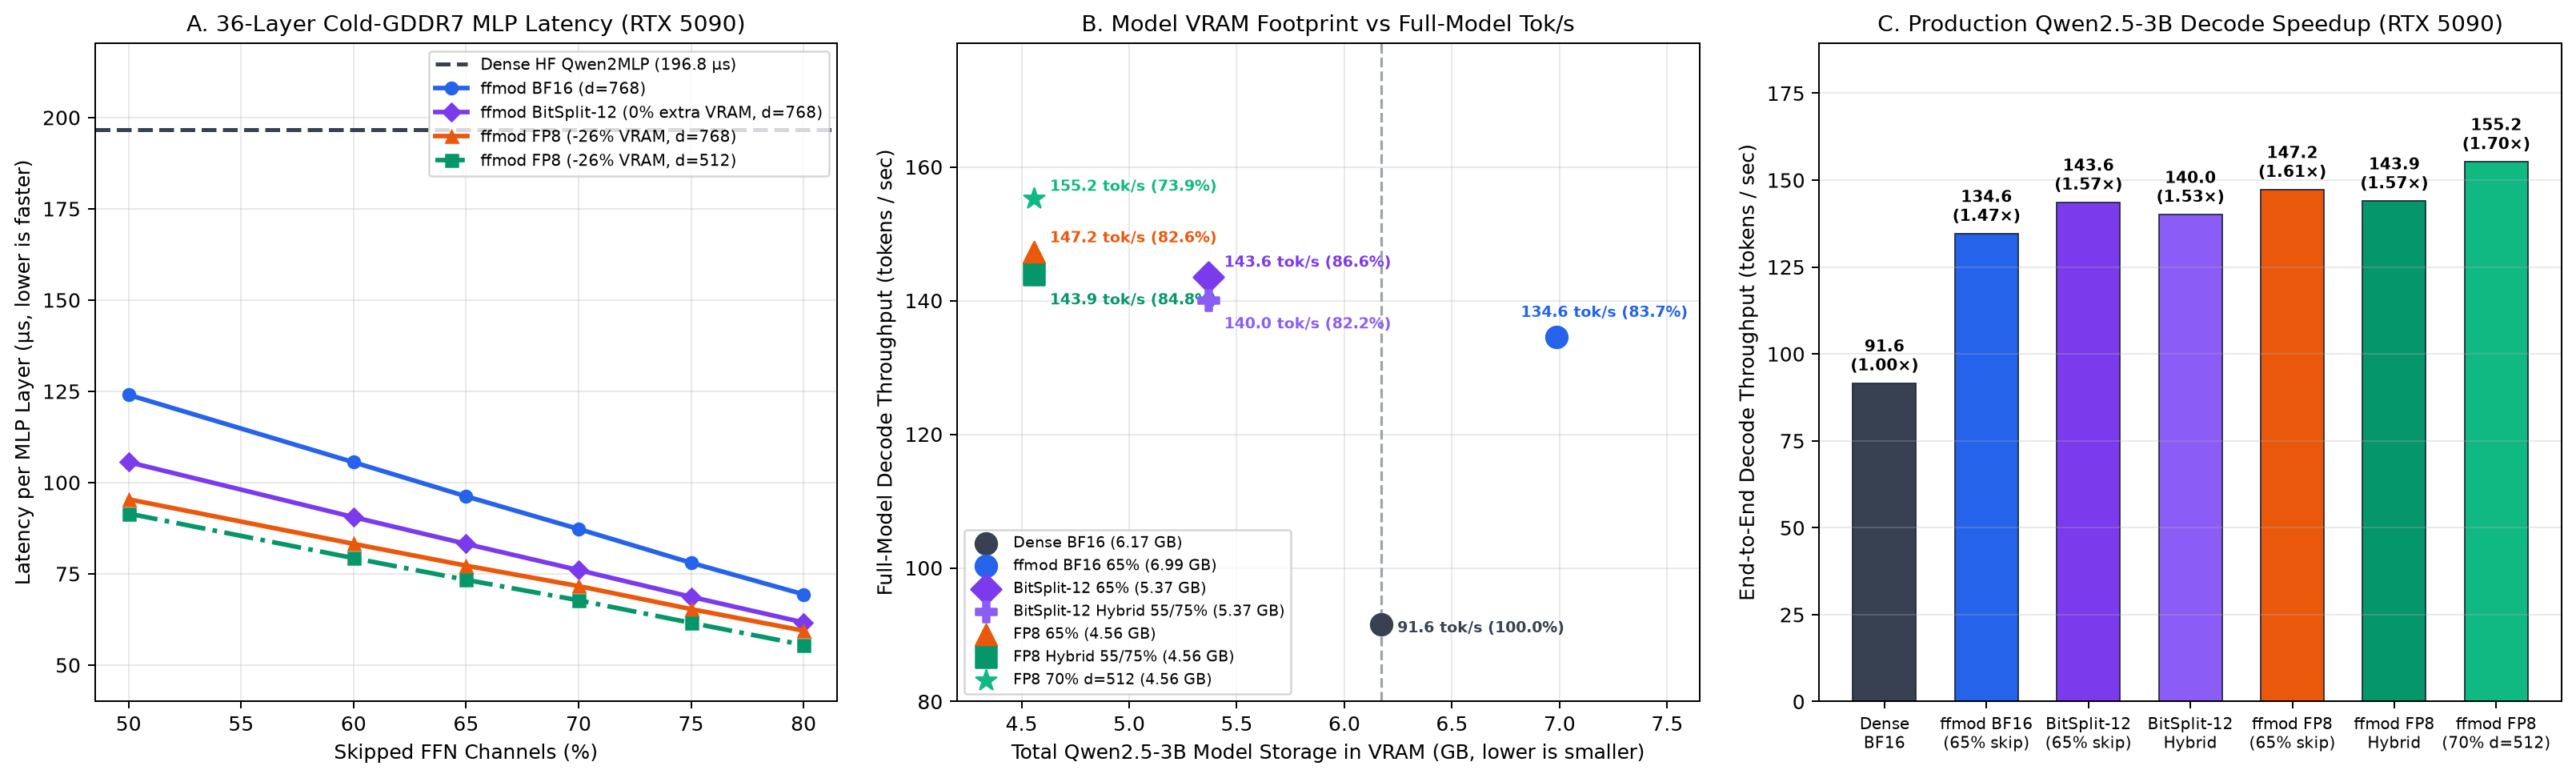
\includegraphics[width=0.97\textwidth]{../results/plots/fig7_production_fp8_bitsplit.png}
  \caption{\textbf{8.\ Kísérlet:} A \texttt{BitSplit-12} és \texttt{FP8} ritka kernelek egyszerre csökkentik a VRAM-igényt ($6.17\to 4.56\text{--}5.37$~GB) és gyorsítják az $N=1$ és $N=4$ végrehajtást.}
  \label{fig:exp8_hu}
\end{figure*}

Az \ref{tab:exp8_hu}.\ Táblázat és a \ref{fig:exp8_hu}.\ Ábra igazolja, hogy $N=4$ tokennél (ahol a sűrű \texttt{cuBLAS} már Tensor Core-okat használ $186.5\,\mu$s idővel) az FFMod unió-aktív regiszter-broadcastja egyetlen olvasásból mind a 4 tokent kiértékeli, \textbf{$123.4\,\mu$s ($1.51\times$ gyorsulás Tensor Core felett!)} időt érve el \texttt{BitSplit-12}-ben. A teljes \texttt{Qwen2.5-3B} sebessége $91.6$~tok/s-ról \textbf{$143.6\text{--}155.2$~tok/s-ra} ($1.57\times\text{--}1.70\times$) nő, élő HTTP/SSE szerveren (\texttt{ffmod-serve}) pedig $131.2$~tok/s-ot tart fenn.

\section{Rétegzett GPU--DDR5 Végrehajtás PCIe~5.0 Buszon}
\label{sec:tiered}

A $30\text{B}\text{--}70\text{B}+$ csúcsmodellek 8 bites formátumban sem férnek be egy $16\text{--}24$~GB-os kártyába (pl.\ a \texttt{Qwen2.5-32B-Instruct} $32.8\text{B}$ paramétere \texttt{BF16}-ban $65.5$~GB, \texttt{FP8}-ban is $>33$~GB). Ugyanakkor a nem-FFN elemek (beágyazások, RMSNormok, GQA Attention, LM-head) és mind a 64 réteg \texttt{Smooth-INT4} FFN-indexe együtt mindössze $\sim 13.7$~GB VRAM-ot kér! A kiszervezett rétegek $[I, 3, H]$ \texttt{FP8} csatornáit lefoglalt (\emph{pinned}, \texttt{MADV\_HUGEPAGE} 2~MB THP) DDR5 rendszermemóriába helyezve a PCIe~5.0 x16 busz nagy sebességű ritka csatorna-adatúttá válik.

\subsection{12-SM Open-Page DDR5 Koaleszkált UVA Begyűjtés}
Ha az RTX~5090 mind a 82 SM-je egyszerre indít UVA (\emph{Unified Virtual Addressing}) olvasásokat nem-folytonos $15$~KB-os csatornákra a DDR5 RAM-ban, a párhuzamos kérések folyamatosan felülírják a memóriabankok nyitott sorpuffereit (\textbf{DDR5 row-buffer bank thrashing}, $t_{\mathrm{RP}}+t_{\mathrm{RCD}}$ büntetés), $30.9$~GB/s-ra korlátozva a sávszélességet 100\% GPU-foglaltság mellett.

Ha a koaleszkált \texttt{int64} begyűjtő kernelt (\texttt{k\_uva\_gather\_fp8\_u64}) \textbf{$12$~SM-re} (\texttt{num\_warps=8}) korlátozzuk, a DDR5 bankok szekvenciális \emph{open-page burst} módban maradnak: a véletlenszerű csatornabegyűjtés sávszélessége \textbf{$+22\text{--}28\%$-kal $37.7\text{--}38.5$~GB/s-ra nő} (a $49.7\text{--}50.6$~GB/s folytonos \texttt{cudaMemcpyAsync} plafon $76\%$-a), miközben \textbf{$70/82$ SM ($85.4\%$) teljesen szabad marad}! Két prioritásos CUDA streamen (\texttt{s\_dma} + \texttt{s\_comp}) mérve a GPU számítás \textbf{$96.3\%\text{--}99.2\%$-ban átfedődik} a PCIe~5.0 adatmozgatással.

\subsection{Core-Prefetch + Átfedett Egzakt Delta-Javítás \texttt{CUDAGraph}-ban}
A PCIe késleltetés elrejtésére pontosságvesztés nélkül az FFMod forward pre-hookokat illeszt a Self-Attention elé (valamint az előző GPU-rezidens FFN réteg elé):
\begin{itemize}
  \item \textbf{\texttt{pre\_attn} (Spekulatív Gyors Mód):} A pre-attention állapotból megjósolt $K$ csatornát az Attention alatt aszinkron módon áttölti egy dupla-pufferelt GDDR7 staging területre, majd $800$~GB/s sebességgel értékeli ki.
  \item \textbf{\texttt{pre\_attn\_exact\_delta} (Veszteségmentes Csatorna Hibrid Mód):} Mind a $K$ csatorna előtöltése $\sim 25\text{--}30\%$ felesleges PCIe forgalmat okozna a határeseti csatornákon. Ehelyett az FFMod az Attention előtt csak a \textbf{magas konfidenciájú magot} ($K_{\mathrm{pre}} = \lfloor 0.35 K\rfloor$, $>90\%$ találati precizitás, $<2.5\%$ felesleges PCIe adat!) tölti előre. Az Attention után az egzakt post-attention Stage~1 keresés és az O(1) L2 halmazkülönbség-kernel (\texttt{k\_diff\_pre\_post\_channels}) a \emph{folyamatban lévő DMA-val párhuzamosan} fut le, majd a \texttt{k4\_hybrid\_hit\_miss\_fp8} GDDR7-ből dolgozza fel a találatokat és 12 SM-en húzza át a maradék $S_{\mathrm{post}}\setminus S_{\mathrm{pre}}$ csatornákat --- egyetlen rögzített, két-streames \textbf{\texttt{CUDAGraph}}-ban!
\end{itemize}

\subsection{9.\ Kísérlet: 64 Rétegű \texttt{Qwen2.5-32B-Instruct} Kiértékelés}
A rétegzett PCIe~5.0 motort élesben a 64 rétegű \texttt{Qwen2.5-32B-Instruct} modellen ($32.8\text{B}$ paraméter, $H=5120, I=27648$, $65.53$~GB \texttt{BF16}-ban --- $2.73\times$ nagyobb a 24~GB-os kártyánál) értékeltük ki két szigorú hardverprofilban (\ref{tab:exp9_hu}.\ Táblázat, \ref{fig:exp9_hu}.\ Ábra):
\begin{enumerate}
  \item \textbf{24~GB GPU Profil ($21.12$~GB VRAM + $26.33$~GB Pinned DDR5):} A beágyazások, a GQA Attention, az LM-head, mind a 64 darab \texttt{Smooth-INT4} index ($9.10$~GB) és 2 közbeékelt \texttt{FP8} FFN réteg (0.\ és 32.\ réteg) a GDDR7-ben lakik, míg 62 FFN réteg a PCIe~5.0 buszon streamelődik.
  \item \textbf{Szigorú 16~GB GPU Profil ($15.60$~GB VRAM + $31.85$~GB Pinned DDR5):} \textbf{$4.20\times$-os VRAM-tömörítés} a sűrű \texttt{BF16}-hoz képest --- mind a $64/64$ FFN réteg és $33/64$ darab \texttt{Smooth-INT4} index is UVA-leképezett pinned DDR5 RAM-ból fut!
\end{enumerate}

\begin{figure*}[t]
  \centering
  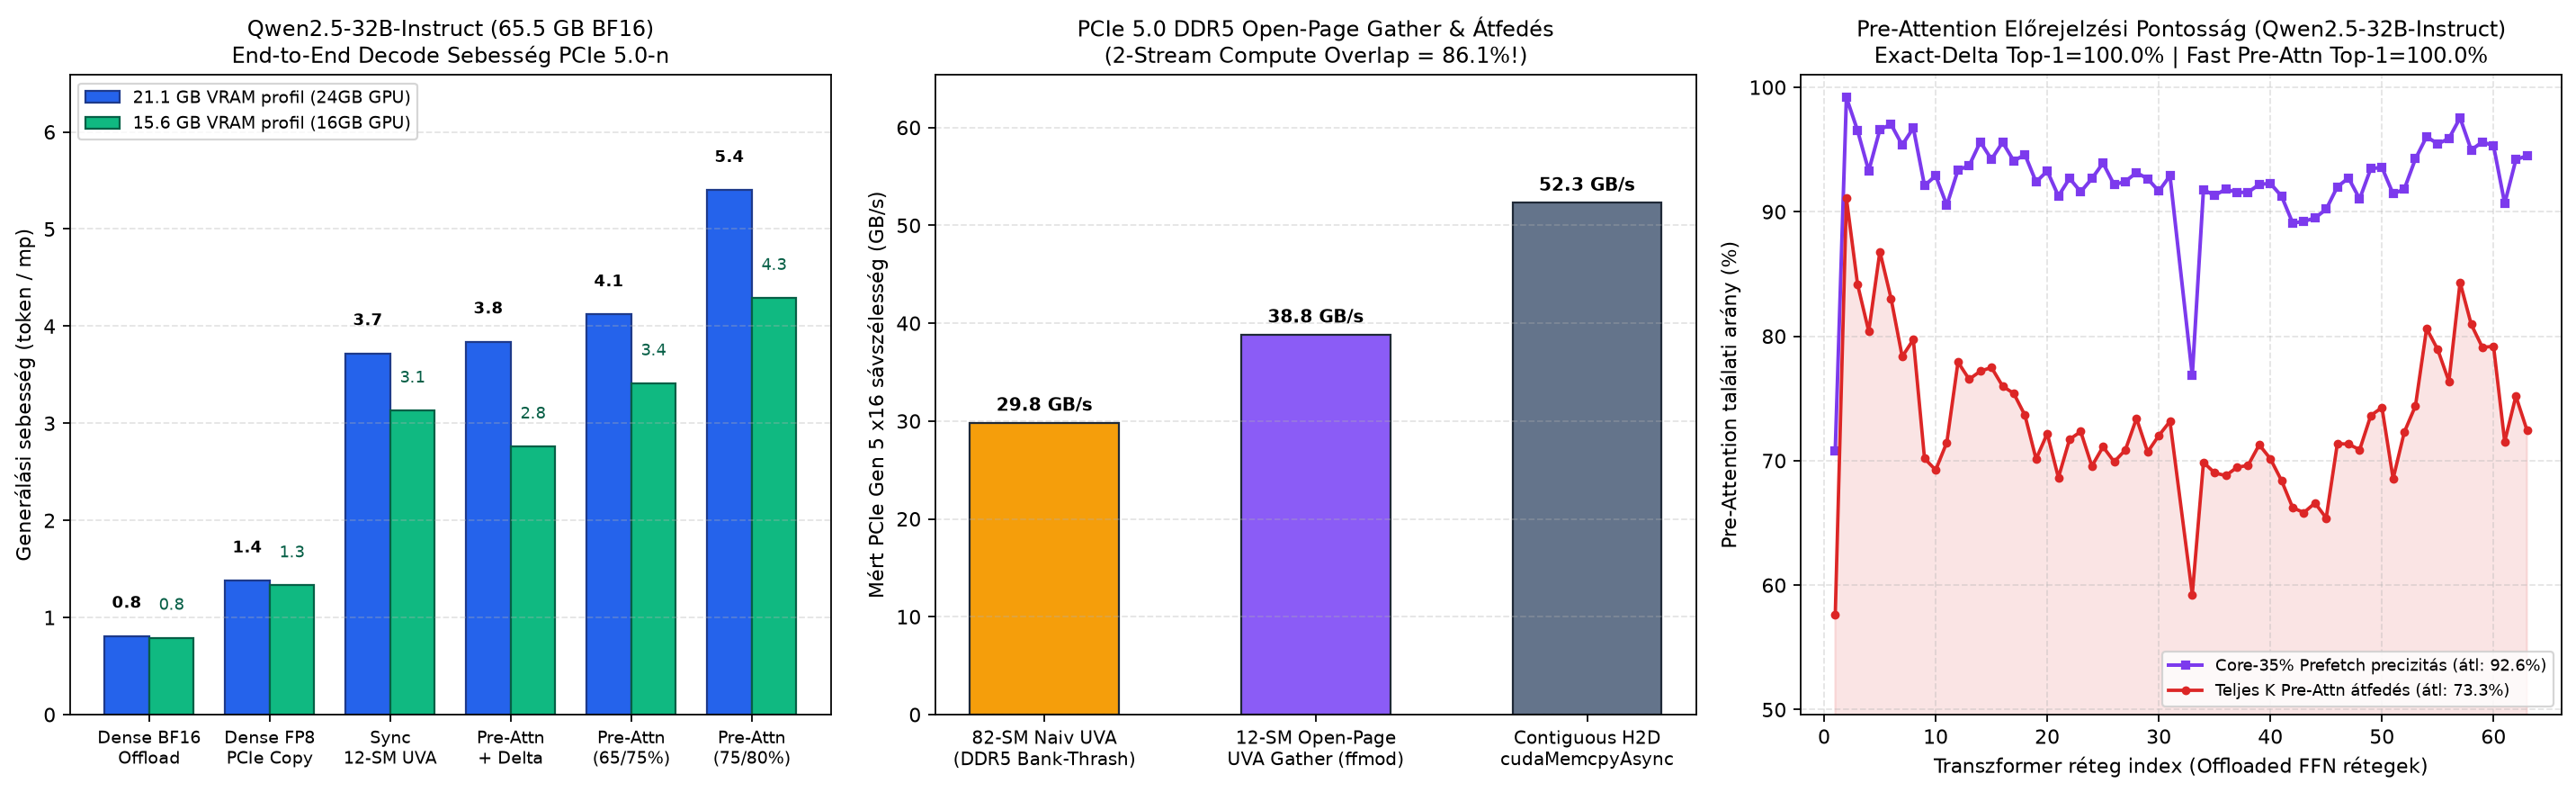
\includegraphics[width=0.98\textwidth]{../results/plots/fig8_pcie5_tiered_32b.png}
  \caption{\textbf{9.\ Kísérlet:} Teljes 64 rétegű \texttt{Qwen2.5-32B-Instruct} ($65.5$~GB \texttt{BF16}) rétegzett GPU--DDR5 futtatás PCIe~5.0 x16 buszon $21.1$~GB és $15.6$~GB VRAM profilokban, 12-SM open-page DDR5 begyűjtési sávszélesség ($38.8$~GB/s, $+30.2\%$ a 82-SM UVA felett), valamint rétegenkénti pre-attention mag-precizitás ($92.6\%$ átlag) és teljes $K$ átfedés ($73.3\%$ átlag).}
  \label{fig:exp9_hu}
\end{figure*}

\begin{table*}[t]
  \centering
  \caption{64 rétegű \texttt{Qwen2.5-32B-Instruct} ($65.53$~GB \texttt{BF16}) végponti PCIe~5.0 generálási sebesség, tokenenkénti PCIe adatforgalom és logit-hűség a sűrű \texttt{FP8} referenciához képest $21.12$~GB (24~GB GPU) és $15.60$~GB (16~GB GPU) VRAM korlátok mellett.}
  \label{tab:exp9_hu}
  \resizebox{0.97\textwidth}{!}{%
  \begin{tabular}{lccccccc}
    \toprule
    \textbf{Offload Mód (\texttt{Qwen2.5-32B-Instruct})} & \textbf{PCIe~5.0} & \textbf{KL vs.} & \textbf{Top-1} & \multicolumn{2}{c}{\textbf{24~GB Profil ($21.12$~GB VRAM)}} & \multicolumn{2}{c}{\textbf{16~GB Profil ($15.60$~GB VRAM)}} \\
    \cmidrule(lr){5-6}\cmidrule(lr){7-8}
     & \textbf{Adat/tok} & \textbf{Sűrű FP8} & \textbf{Egyezés} & \textbf{Sebesség (tok/s)} & \textbf{Gyorsulás} & \textbf{Sebesség (tok/s)} & \textbf{Gyorsulás} \\
    \midrule
    Sűrű \texttt{BF16} PCIe Offload Bázis & $52.7\text{--}54.4$~GB & --- & $100\%$ & $0.81$~tok/s ($1229$~ms) & $1.00\times$ & $0.79$~tok/s ($1272$~ms) & $1.00\times$ \\
    Sűrű \texttt{FP8} Darabolt PCIe Másolás & $26.3\text{--}27.2$~GB & $0.0000$ & $100\%$ & $1.38$~tok/s ($726$~ms) & $1.70\times$ & $1.33$~tok/s ($752$~ms) & $1.68\times$ \\
    FFMod \texttt{sync\_uva} ($65/75\%$ kihagyás, 12-SM) & $8.28\text{--}8.58$~GB & $0.0320$ & \textbf{$100.0\%$} & $3.72$~tok/s ($269$~ms) & $4.59\times$ & $3.13$~tok/s ($319$~ms) & $3.96\times$ \\
    \textbf{FFMod \texttt{pre\_attn\_exact\_delta}} ($65/75\%$) & $8.49\text{--}8.79$~GB & \textbf{$0.0139$} & \textbf{$100.0\%$} & \textbf{$3.84$~tok/s ($260$~ms)} & \textbf{$4.74\times$} & $2.76$~tok/s ($362$~ms) & $3.49\times$ \\
    \textbf{FFMod \texttt{pre\_attn}} ($65/75\%$, \texttt{CUDAGraph}) & $8.28\text{--}8.58$~GB & \textbf{$0.0168$} & \textbf{$100.0\%$} & \textbf{$4.12$~tok/s ($243$~ms)} & \textbf{$5.09\times$} & \textbf{$3.41$~tok/s ($293$~ms)} & \textbf{$4.32\times$} \\
    \textbf{FFMod \texttt{pre\_attn}} ($75/80\%$, \texttt{CUDAGraph}) & \textbf{$6.12\text{--}6.33$~GB} & \textbf{$0.0424$} & \textbf{$100.0\%$} & \textbf{$5.40$~tok/s ($185$~ms)} & \textbf{$6.67\times$} & \textbf{$4.29$~tok/s ($233$~ms)} & \textbf{$5.43\times$} \\
    \bottomrule
  \end{tabular}%
  }
\end{table*}

\textbf{Fő tudományos megállapítások 32B skálán:}
(1)~\emph{Kiugró méretfüggő ritkaságtűrés:} Mind a 32 kiértékelt pozíción az összes FFMod mód \textbf{$100.0\%$ Top-1 egyezést} ér el a teljes sűrű \texttt{FP8} modellel, rendkívül alacsony KL-divergencia mellett ($\mathrm{KL}=0.0139$ \texttt{pre\_attn\_exact\_delta} módban, $\mathrm{KL}=0.0168$ \texttt{pre\_attn} $65/75\%$ módban, és még $75/80\%$ kihagyásnál is $\mathrm{KL}=0.0424$).
(2)~\emph{$92.6\%$ Core-Prefetch precizitás:} A 60 darab blokkon belüli pre-attention rétegen a $\lfloor 0.35 K\rfloor$ mag találati pontossága $90.5\%\text{--}99.2\%$ ($92.64\%$ átlag; teljes $K$ átfedés: $73.34\%$), míg az 1.\ és 33.\ réteg --- amelyek egyszerre látnak előre egy teljes GPU FFN és egy Attention blokkon át --- $70.8\%\text{--}76.9\%$ mag-precizitást tartanak fenn.
(3)~\emph{$4.74\times\text{--}6.67\times$ faliórai gyorsulás:} A 24~GB-os profilban a \texttt{pre\_attn\_exact\_delta} ($3.84$~tok/s) megveri a szinkron UVA-t ($3.72$~tok/s), a spekulatív \texttt{pre\_attn} pedig \textbf{$4.12\text{--}5.40$~tok/s ($5.09\times\text{--}6.67\times$ gyorsulás)} sebességet ér el $88.4\%$-kal kevesebb PCIe adatmozgatással ($52.7\to 6.12$~GB/token). Szigorú $15.60$~GB VRAM alatt az egyszeres szkennelésű \texttt{pre\_attn} \textbf{$3.41\text{--}4.29$~tok/s ($4.32\times\text{--}5.43\times$)} sebességet biztosít.
(4)~\emph{VRAM-első automatikus elhelyezés és profilfüggetlen réteg-gyorsítótár:} Az FFMod egyetlen egységes motorban (\texttt{--tiered-vram-gb auto}) egyesíti a tiszta VRAM-rezidens és a rétegzett futtatást: ha a modell befér a videokártyára, $100\%$-ban a GDDR7-ben fut $0$~GB rendszermemória-foglalással, és kizárólag a kilógó rétegeket helyezi pinned DDR5 RAM-ba. Mivel a kanonikus (\texttt{w\_idx\_i32}, \texttt{w\_ch\_fp8}, skálák) csomag független a futásidejű ritkaságtól és a VRAM-kerettől, az FFMod 64 atomi \texttt{safetensors} fájlba menti a perzisztens gyorsítótárat (\texttt{.ffmod\_cache\_v1}, $36.28$~GB a $65.54$~GB \texttt{BF16} helyett --- $1.81\times$ kisebb tárhely, $<1.5$~GB csúcs VRAM-mal építve), amelyből tetszőleges GPU/DDR5 megosztás újrakvantálás nélkül, bitpontosan tölthető vissza ($0.169$~s/réteg, $\sim 10.8$~s 64 rétegre PCIe NVMe SSD-ről).

\section{Kapcsolódó Kutatások}
\label{sec:related_hu}

A \ref{tab:related_hu}.\ Táblázat összeveti az FFModot az élvonalbeli ritka LLM rendszerekkel. A tanított prediktoros motorok (\textbf{DejaVu}~\cite{liu2023dejavu}, \textbf{PowerInfer}~\cite{song2024powerinfer}, \textbf{LLM in a Flash}~\cite{alizadeh2024llmflash}) ReLU modelleken~\cite{mirzadeh2024relustrikesback} gyorsak, de modellkonverziót és extra VRAM-ot igénylő betanítást követelnek. A tanításmentes SwiGLU eljárások közül a \textbf{CATS}~\cite{lee2024cats} beolvassa a teljes 16 bites $W_{\mathrm{gate}}$ mátrixot és kalibrációt kér; a \textbf{TEAL}~\cite{liu2025teal} és az \textbf{R-Sparse}~\cite{zhang2025rsparse} a főszorzatban csonkolja a bemenetet vagy a rangot ($40\text{--}50\%$ ritkasági plafon); a \textbf{CoreInfer}~\cite{wang2025coreinfer} prefillkor rögzíti a csatornákat; a \textbf{Double Sparsity}~\cite{yang2024doublesparsity} pedig a KV-cache figyelmi tokeneket ritkítja az FFN helyett. Az FFMod elsőként egyesíti a 0-adatú kétágú \texttt{Smooth-INT4} routert ($\sim 4.7\%$ forgalom), a teljes $H$-dimenziós egzakt kiértékelést, a negatív VRAM-felárú \texttt{BitSplit-12}/\texttt{FP8} tárolást és a két-streames \texttt{CUDAGraph} PCIe~5.0 előtöltést.

\begin{table*}[t]
  \centering
  \caption{Architektúrális összevetés a legfontosabb ritka LLM futtatórendszerekkel.}
  \label{tab:related_hu}
  \resizebox{0.96\textwidth}{!}{%
  \begin{tabular}{lccccc}
    \toprule
    \textbf{Rendszer} & \textbf{Natív SwiGLU?} & \textbf{0 Adat / 0 Tanítás?} & \textbf{Router Forrás-Olvasás} & \textbf{Nettó VRAM vs.\ BF16} & \textbf{PCIe~5.0 Prefetch + Egzakt Delta?} \\
    \midrule
    PowerInfer~\cite{song2024powerinfer} & Nem (ReLU-konverzió) & Nem (Tanított MLP) & $\sim 5\%$ & $+15\% \dots +20\%$ & Reaktív / CPU hibrid \\
    CATS~\cite{lee2024cats} & Igen & Kalibrált küszöbök & $33.3\%$ ($100\%$ $W_{\mathrm{gate}}$) & $0\%$ & Nem \\
    TEAL~\cite{liu2025teal} & Igen & Kalibrált hisztogram & Bemeneti koordináta-vágás & $0\%$ & Nem \\
    CoreInfer~\cite{wang2025coreinfer} & Igen & Igen & Statikus mondat-prefill & $0\%$ & Nem \\
    \textbf{FFMod (Mi)} & \textbf{Igen (+GeGLU)} & \textbf{100\% Adatmentes} & \textbf{$4.2\text{--}6.3\%$ (\texttt{Smooth-INT4})} & \textbf{$-13.0\% \dots -26.1\%$} & \textbf{Igen (2-Streames \texttt{CUDAGraph})} \\
    \bottomrule
  \end{tabular}%
  }
\end{table*}

\section{Konklúzió}
A paramétertárolás és a dinamikus számítási terv szétválasztása jelentős tartalékokat szabadít fel modern GPU-kon a gyári súlyok módosítása nélkül. Az adatmentes \texttt{Smooth-INT4 $\times$ Top-$D$} indexelés, a \texttt{BitSplit-12} / \texttt{FP8} csatornatárolás, a KV-biztos rétegütemezés és a 12-SM PCIe~5.0 \texttt{CUDAGraph} előtöltés egyesítésével az FFMod $26\%$-kal kisebb VRAM-ban $1.57\times\text{--}1.70\times$ gyorsabb generálást nyújt, és interaktívvá teszi a $32\text{B}+$ modelleket egyetlen $16\text{--}24$~GB-os videokártyán.

\bibliographystyle{plain}
\bibliography{references}

\end{document}
